Dans cet exercice, toutes les questions et sous-questions sont, dans une large mesure, indépendantes. Certaines montrent crescendo en difficulté. Toutes les réponses devront être argumentées.

\medskip

\noindent
\section*{1. Les feux de l'amour.} 
Si Alice n'aime pas Jordan alors Brenda n'aime pas Dan. 
Si Brenda aime Jordan, alors Alice n'aime pas Jordan. 
Si Brenda n'aime pas Jordan, alors Brenda n'aime pas Dan. 
Brenda aime-t-elle Dan ?

\medskip

\noindent
\section*{2. Retour vers le futur.} 
Votre oncle a 54 ans. En échangeant les chiffres des unités et des dizaines, il n'a plus que 45 ans. Cet artifice lui fait gagner 9 ans. 
Plus généralement, envisageons une personne ayant \( ab \) années, avec éventuellement \( a = 0 \) (dans l'exemple ci-dessus, \( a = 5 \) et \( b = 4 \)).  
\begin{enumerate}
    \item Combien d'années, au maximum, cette facétieuse personne pourrait-elle gagner grâce à ce procédé ?  
    \item Cette personne pourrait-elle ainsi gagner exactement 30 ans ?
\end{enumerate}

\medskip

\noindent
\section*{3. Intelligence Administrative.} 
4 personnes se présentent à l'élection d'un conseil. Tous les votes sont valides et exprimés. Voici les résultats obtenus : 
Johanna obtient \( \frac{1}{4} \) des voix, Jason obtient \( \frac{4}{15} \) des voix, Jasmine obtient \( \frac{3}{20} \) des voix, et Julie obtient \( \frac{1}{3} \) des voix. 
Qui l'emporte et combien pouvait-il y avoir de votants ?

\medskip

\noindent
\section*{4. Une moitié de seau pas si bête.} 
Un seau a la forme d'un tronc de cône de petit rayon \( r \), de grand rayon \( R > r \) et de hauteur totale \( h \).  

\begin{enumerate}
    \item Justifier que son volume total vaut  
    \[
    V = \frac{\pi h}{3} \bigl( r^2 + Rr + R^2 \bigr).
    \]

    \begin{minipage}{.5\linewidth}
    \item On remplit le seau jusqu'à la hauteur \( x \), nombre réel appartenant à l'intervalle \([0, h]\). 
    La surface de l'eau à cette hauteur est un disque de rayon \( \rho \). 
    Déterminer \( \rho \) à l'aide de \( x, r, R \) et \( h \).

    \item On suppose que \( r = 1,\; R = 1,2 \) et \( h = 2 \). 
    À l'aide de votre calculatrice, donner une valeur approchée de \( x \) de sorte que le seau soit rempli à la moitié de sa capacité. \\
    Pourquoi pouvait-on limiter la recherche autour et au-dessus de la valeur \( x = 1 \) ?
    \end{minipage}
    \hfill\begin{minipage}{.5\linewidth}
    \begin{center}
    \begin{tikzpicture}[line width=1pt, scale=0.5]
    % Remplissage à moitié avec des motifs de vaguelettes
    % La moitié correspond à une hauteur de 3.5 sur 7
    \fill[pattern=north east lines, pattern color=blue!40] 
        (0,0) -- (-.6,4.2) -- (6.6,4.2) -- (6,0) -- cycle;
    
    % Trait du verre (par-dessus pour bien délimiter)
    \draw[] (0,0) -- (-1,7) -- (7,7) -- (6,0) -- cycle;
    
    % Lignes verticales pour matérialiser les mesures
    \draw[dashed, thin, gray] (3,-.5) -- (3,7.5);
    \draw[dashed, thin, gray] (6,-.5) -- (6,0);
    \draw[dashed, thin, gray] (6.6,3.7) -- (6.6,4.8);
    \draw[dashed, thin, gray] (7,6.5) -- (7,7.5);
    
    %Flèches horizontales pour matérialiser les mesures
    \draw[<->, thin, gray] (3,-.25) -- (6,-0.25) node[midway, below] {$r$};
    \draw[<->, thin, gray] (3,4.45) -- (6.6,4.45) node[midway, above] {$\rho$};
    \draw[<->, thin, gray] (3,7.25) -- (7,7.25) node[midway, above] {$R$};
    
    % Lignes horizontales pour matérialiser les mesures
    \draw[dashed, thin, gray] (6,0) -- (9,0);
    \draw[dashed, thin, gray] (6.6,4.2) -- (8,4.2);
    \draw[dashed, thin, gray] (7,7) -- (9,7);
    
    %Flèches verticales pour matérialiser les mesures
    \draw[<->, thin, gray] (7.5,0) -- (7.5,4.2) node[midway, right] {$x$};
    \draw[<->, thin, gray] (8.5,0) -- (8.5,7) node[midway, right] {$h$};
    \end{tikzpicture}
    \end{center}
    \end{minipage}
    
    
\end{enumerate}

\section*{5. Triominos. } 
Les polygones suivants, formés de trois carrés, sont appelés \textit{triominos} :
\begin{center}
\begin{center}
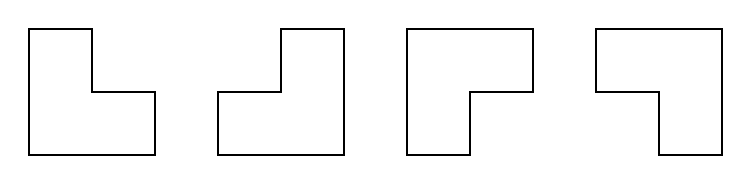
\begin{tikzpicture}[line width=1pt, scale=0.8]
% L n°2 : rotation 90°
\begin{scope}[shift={(0,0)}]
\draw[rotate=90] (0,0) -- (1,0) -- (1,1) -- (2,1) -- (2,2) -- (0,2) -- cycle;
\end{scope}

% L n°3 : rotation 180°
\begin{scope}[shift={(3,2)}]
\draw[rotate=180] (0,0) -- (1,0) -- (1,1) -- (2,1) -- (2,2) -- (0,2) -- cycle;
\end{scope}
% L n°1 : rotation 0° (original)
\begin{scope}[shift={(4,0)}]
\draw (0,0) -- (1,0) -- (1,1) -- (2,1) -- (2,2) -- (0,2) -- cycle;
\end{scope}
% L n°4 : rotation 270° (ou -90°)
\begin{scope}[shift={(7,2)}]
\draw[rotate=270] (0,0) -- (1,0) -- (1,1) -- (2,1) -- (2,2) -- (0,2) -- cycle;
\end{scope}
\end{tikzpicture}
\end{center}
\end{center}

\begin{minipage}{.65\linewidth}
On s'intéresse au pavage par des triominos de grilles (ou, en b. et c. de morceaux de grilles) de format \( a \times b \), où \( a \) désigne leur nombre de lignes et \( b \) leur nombre de colonnes. La figure ci-contre montre un exemple de pavage d'une grille dans le cas où \( a = 2 \) et \( b = 6 \).
\end{minipage}
\hfill\begin{minipage}{.35\linewidth}
\begin{center}
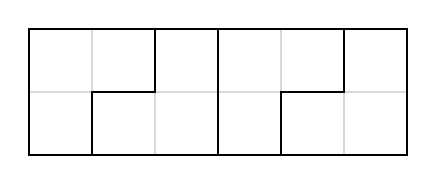
\begin{tikzpicture}[line width=1pt, scale=0.8]% Grille grise en arrière-plan
\draw[gray!30, step=1] (0,0) grid (6,2);
% L n°3 : rotation 180°
\begin{scope}[shift={(3,2)}]
\draw[rotate=180] (0,0) -- (1,0) -- (1,1) -- (2,1) -- (2,2) -- (0,2) -- cycle;
\end{scope}
% L n°1 : rotation 0° (original)
\begin{scope}[shift={(0,0)}]
\draw (0,0) -- (1,0) -- (1,1) -- (2,1) -- (2,2) -- (0,2) -- cycle;
\end{scope}

% L n°3 : rotation 180°
\begin{scope}[shift={(6,2)}]
\draw[rotate=180] (0,0) -- (1,0) -- (1,1) -- (2,1) -- (2,2) -- (0,2) -- cycle;
\end{scope}
% L n°1 : rotation 0° (original)
\begin{scope}[shift={(3,0)}]
\draw (0,0) -- (1,0) -- (1,1) -- (2,1) -- (2,2) -- (0,2) -- cycle;
\end{scope}
\end{tikzpicture}
\end{center}
\end{minipage}

\medskip

Soit \( n \) un entier naturel non nul.

\begin{minipage}{.65\linewidth}
\begin{enumerate}
\item Est-il possible de paver une grille de format \( 2^n \times 2^n \) ?
\item On retire le carré en haut à gauche d'une telle grille (exemple ci-contre avec \( n = 2 \)). Démontrer qu'il est alors possible de paver cette grille ainsi modifiée (on commencera par les cas \( n = 1 \) et \( n = 2 \) avant de généraliser).
\item Démontrer que le résultat précédent reste vrai quand on enlève n'importe laquelle des cases de la grille complète \( 2^n \times 2^n \) initiale.
\end{enumerate}
\end{minipage}
\hfill\begin{minipage}{.35\linewidth}
\begin{center}

\begin{tikzpicture}[line width=1pt, scale=0.8]% Grille grise en arrière-plan
\draw[gray!30, step=1] (0,0) grid (4,4);
\draw[white] (0,3) -- (0,4) -- (1,4) ;
\end{tikzpicture}
\end{center}
\end{minipage}



\section*{6. Sommes harmoniques.}

Pour \( n \) entier naturel, \( n \geqslant 1 \), on calcule la somme (dite « harmonique »)
\[
H_n = 1 + \frac{1}{2} + \frac{1}{3} + \cdots + \frac{1}{n}.
\]
Ainsi, \( H_1 = 1 \), \( H_2 = 1 + \frac{1}{2} = \frac{3}{2} \), \( H_3 = 1 + \frac{1}{2} + \frac{1}{3} = \frac{11}{6} \).

\begin{enumerate}
\item Justifier que \( H_4 = \frac{25}{12} \).
\item Proposer un code en langage Python permettant d'obtenir \( H_n \) pour tout entier naturel \( n \) avec \( n \geqslant 1 \).
\item On appelle « terme binaire » de \( H_n \) l'inverse de la plus grande puissance de deux figurant parmi ses termes à sommer. Ainsi, le terme binaire de \( H_2 \) est \( \frac{1}{2} \), celui de \( H_3 \) aussi ; le terme binaire de \( H_8 \) est \( \frac{1}{8} \), celui de \( H_9 \), de \( H_{10} \), \ldots, \( H_{15} \) aussi, etc. Quel est le terme binaire de \( H_3 \) ? De \( H_5 \) ? De \( H_{20} \) ?
\item On remarque, après quelques essais, que les valeurs de \( H_n \) ne semblent jamais être entières dès que \( n \geqslant 2 \). Démontrer-le à l'aide, notamment, du terme binaire de \( H_n \).
\end{enumerate}
